% Unofficial University of Cambridge Poster Template
% https://github.com/andiac/gemini-cam
% a fork of https://github.com/anishathalye/gemini
% also refer to https://github.com/k4rtik/uchicago-poster

\documentclass[final]{beamer}

% ====================
% Packages
% ====================

\usepackage[T1]{fontenc}
\usepackage{lmodern}
\usepackage[size=custom,width=91.44,height=60.96,scale=0.9]{beamerposter}
\usetheme{gemini}
\usecolortheme{uchicago}
% 36x24in is narrower than the template default, so the title column is tighter.
% One step down from the theme default (\Huge) keeps the title on two lines.
\setbeamerfont{headline title}{size=\huge,series=\bfseries}
\usepackage{graphicx}
\usepackage{booktabs}
\usepackage[numbers]{natbib}
\usepackage{tikz}
\usepackage{pgfplots}
\pgfplotsset{compat=1.14}
\usepackage{anyfontsize}

% ====================
% Lengths
% ====================

% If you have N columns, choose \sepwidth and \colwidth such that
% (N+1)*\sepwidth + N*\colwidth = \paperwidth
\newlength{\sepwidth}
\newlength{\colwidth}
\setlength{\sepwidth}{0.025\paperwidth}
\setlength{\colwidth}{0.3\paperwidth}

\newcommand{\separatorcolumn}{\begin{column}{\sepwidth}\end{column}}

% ====================
% Title
% ====================

% Line break is manual: beamerposter does not wrap the title automatically.
% The short title in [] is what goes into the PDF metadata -- without it,
% hyperref hits the \\ while building the metadata string and errors out.
\title[Graph Neural Network Modeling of Breast MRI Vascular Networks for Treatment Response Prediction]{Graph Neural Network Modeling of Breast MRI Vascular \\ Networks for Treatment Response Prediction}

\author{Spencer Venancio \inst{1} \and Advisor: Anna Woodard, PhD \inst{2}}

\institute[shortinst]{\inst{1} University of Wisconsin--Madison \samelineand
  \inst{2} Data Science Institute, University of Chicago}

% ====================
% Footer (optional)
% ====================

% TODO: fill in before printing. Left as visible TODOs rather than the upstream
% example.com/"ABC Conference" placeholders, which look real enough to survive
% to the printer by accident.
\footercontent{
 github.com/dsi-clinic/vanguard \hfill
  University of Chicago Data Science Institute Summer Research Symposium \hfill
  svenancio@wisc.edu}
% (this whole block can be deleted to remove the footer)

% ====================
% Logo (optional)
% ====================

% Three logos: two on the left, one on the right.
%
% Provenance -- all official, all with real alpha:
%   uchicago_seal_white.png  Seal.zip, PNG_RGB_Digital/UChicago_ReverseSeal_
%                            1Color_White_RGB.png
%   uchicago_logo_white.png  University-Logo.zip, PNG_RGB_Digital/Reverse
%                            University Logo_1Color_White_RGB.png (spare: the
%                            shield+wordmark lockup, which UChicago's guidelines
%                            prefer over the seal for general communications)
%                            both from https://creative.uchicago.edu/logos-and-identity-elements
%   dsi_logo_white.pdf       https://datascience.uchicago.edu/wp-content/uploads/
%                            2023/01/DSI_Logo_Color@1x.svg
%   dsi_logo_color.pdf       .../DSI_Logo_Color-2@1x.svg (spare, colour version)
%
% The DSI filenames are misleading: DSI_Logo_Color@1x.svg is entirely #FFFFFF
% (the knockout the DSI site uses on its dark footer); DSI_Logo_Color-2@1x.svg
% is the actual colour one (#8B0021 + #58595B). Converted SVG -> PDF with
% `rsvg-convert -f pdf`, so they stay vector at print size.
%
% The "Reverse ... White" variants are the knockout versions, meant for dark
% backgrounds -- which is what the maroon headline needs. Do not swap in the
% colour DSI logo without also lightening the headline: its maroon ink is
% RGB(139,0,33) against a RGB(128,0,0) bar, so it disappears.
%
% Two constraints worth keeping if you swap these:
%   - The theme reserves \maxlogowidth on BOTH sides of the title, taking the
%     wider of the two sides. A wide logo block on one side eats into the title
%     twice over, squeezing it towards one word per line.
%   - Do not use .eps. An EPS logo makes lualatex exit nonzero even though the
%     PDF comes out fine, which then wedges latexmk. PNG and PDF are both fine.
\logoleft{%
  \begin{tabular}{@{}l@{}}
    
\includegraphics[height=5.5cm]{logos/uchicago_logo_white.png} \\[1.5ex]
    
\includegraphics[height=4.6cm]{logos/dsi_logo_white.pdf}
  \end{tabular}%
}
\logoright{
\includegraphics[height=6.9cm]{logos/uw_madison_white.pdf}}

% ====================
% Body
% ====================

\begin{document}

% Note: the upstream template placed its logo here as an absolutely-positioned
% tikzpicture overlay, which sits on top of the headline instead of inside it --
% so a title of any length runs straight through the logo. That is why the logos
% are set with the theme's own \logoleft/\logoright hooks in the preamble
% instead: those reserve space and keep the title clear of them.

\begin{frame}[t]
\begin{columns}[t]
\separatorcolumn

\begin{column}{\colwidth}

  \begin{block}{Introduction + Motivation}

    Breast cancer is the most common cancer in women worldwide,
    and for those diagnosed with locally advanced breast cancer (LABC), 
    neoadjuvant chemotherapy (NAC) is the standard of care. 
    However, only 30\% of patients achieve a \textbf{pathologic complete response (pCR)}
    to NAC, which is associated with improved survival outcomes. NAC is an 
    intensive treatment that can have significant side effects, and 
    patients who do not achieve pCR may require additional treatment. We would 
    like to develop methods to predict which patients will respond to NAC,
    so that we can better tailor treatment plans and improve outcomes for 
    patients with LABC.
     
  \end{block}

  \begin{block}{Ultrafast MRI Dataset}

    The dataset used in this study consists of \textbf{ultrafast breast MRI} scans from
    $n=100$ patients with LABC who underwent NAC. The scans were acquired using a 
    3T MRI scanner and included both pre- and post-contrast images. The dataset
    also includes clinical information such as age, tumor size, and hormone 
    receptor status, as well as treatment response data (pCR vs. non-pCR).

  \end{block}

  \begin{alertblock}{Graph Representation}

    \begin{figure}
      \centering
      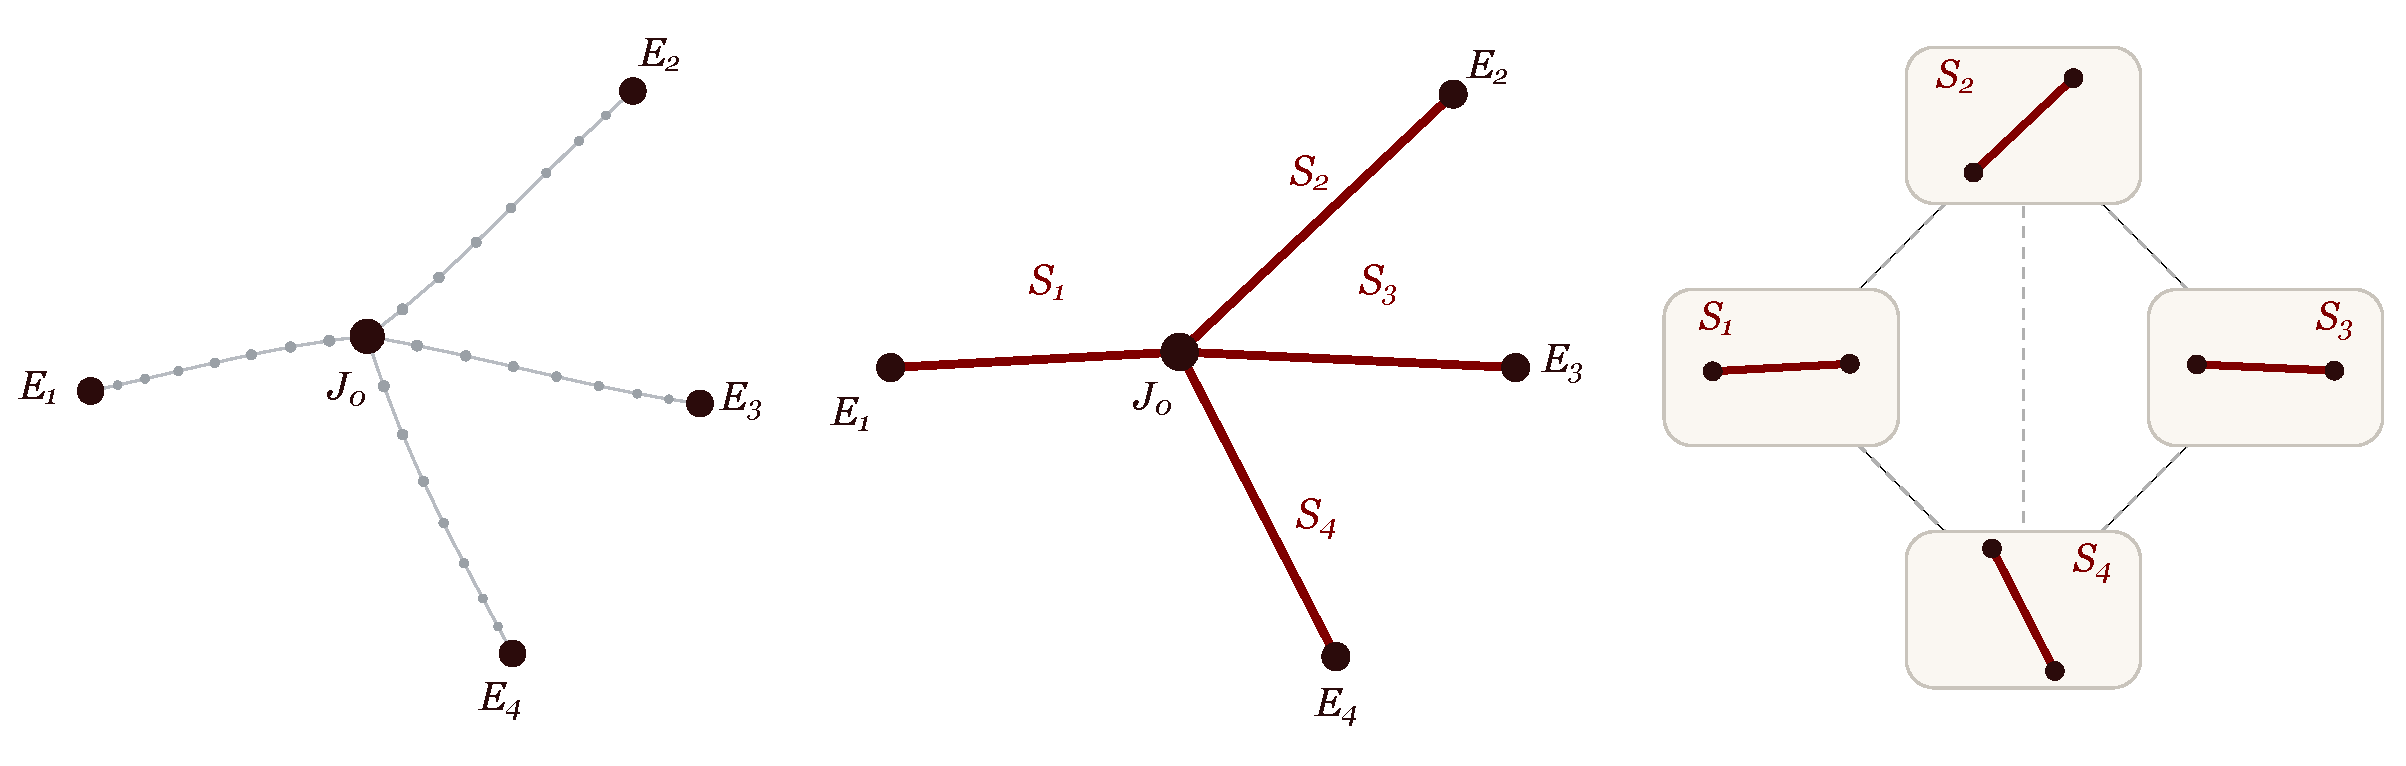
\includegraphics[width=0.75 \linewidth]{figures/graph_representation.pdf}
      \caption{Vascular segments and junctions are converted into graph nodes
      and edges.}
    \end{figure}

    We represent the vascular network of each patient's tumor as a graph, and 
    propose 3 different methods of constructing the graph from the MRI scans.
    In the following let $\mathcal{G} = (\mathcal{V}, \mathcal{E})$ be a graph.

    \begin{itemize}
      \item  \textbf{Voxel-as-node} Let the set of nodes $\mathcal{V}_{\text{vox}}$ be the set 
      of all voxels, and let the set of edges $\mathcal{E}_{\text{vox}}$
      be the set of all pairs of adjacent voxels. In this representation, each 
      voxel is a node, and edges connect adjacent voxels.

       \item \textbf{Junction-as-node} Let $\mathcal{V}_{\text{jun}}$ be the 
       set of all junctions (i.e. $e \in \mathcal{E}_{\text{vox}}$ with $\mathrm{deg}(e) > 2$) 
       in the vascular network, and let $\mathcal{E}_{\text{jun}}$ be the set
       of all pairs of junctions that are connected by a vascular segment.

       \item \textbf{Segement-as-node} Let $\mathcal{V}_{\text{seg}}$ be the 
       set of all vascular segments, and let $\mathcal{E}_{\text{seg}}$ be the 
       set of all pairs of segments that are connected at their endpoints. In this 
       representation, each segment is a node, and edges connect adjacent segments.
     
    \end{itemize}
  \end{alertblock}

\end{column}

\separatorcolumn

\begin{column}{\colwidth}

  % Pipeline and architecture are one block: the two used to end and begin with
  % the same sentence ("a GNN is trained to predict treatment response from the
  % graph representation"), and each figure carries most of its own explanation.
  % Merging them frees a block header and about eighty words for the pretext-task
  % section below.
  \begin{block}{Prediction Pipeline and GNN Architecture}

    \begin{figure}
      \centering
      
\includegraphics[width=\linewidth]{figures/dsi-pipeline.pdf}
      \caption{End-to-end prediction pipeline.}
    \end{figure}

    Vessel segmentation is performed using a \textbf{nnU-Net model}, which labels
    each voxel as vessel or background. The segmentation is simplified into a
    one-voxel wide network of vessels using the \textbf{tc4d} algorithm, then
    converted into a graph using one of the three representations above.

    A \textbf{Graph Neural Network (GNN)} predicts treatment response from that
    graph. Successive \textbf{graph convolution (GCN)} layers aggregate information
    from neighboring nodes, a global pooling layer collapses all nodes into a
    fixed-size representation of the entire graph, and a fully connected layer maps
    that representation to a binary prediction (pCR vs. non-pCR).

    % Vector PDF (25.3 x 9.1 cm, no raster layers), so it scales cleanly. Figure
    % text scales with the include width, not the poster size: at 0.4\textwidth
    % these labels rendered at roughly 40% of the size drawn.
    \begin{figure}
      \centering
      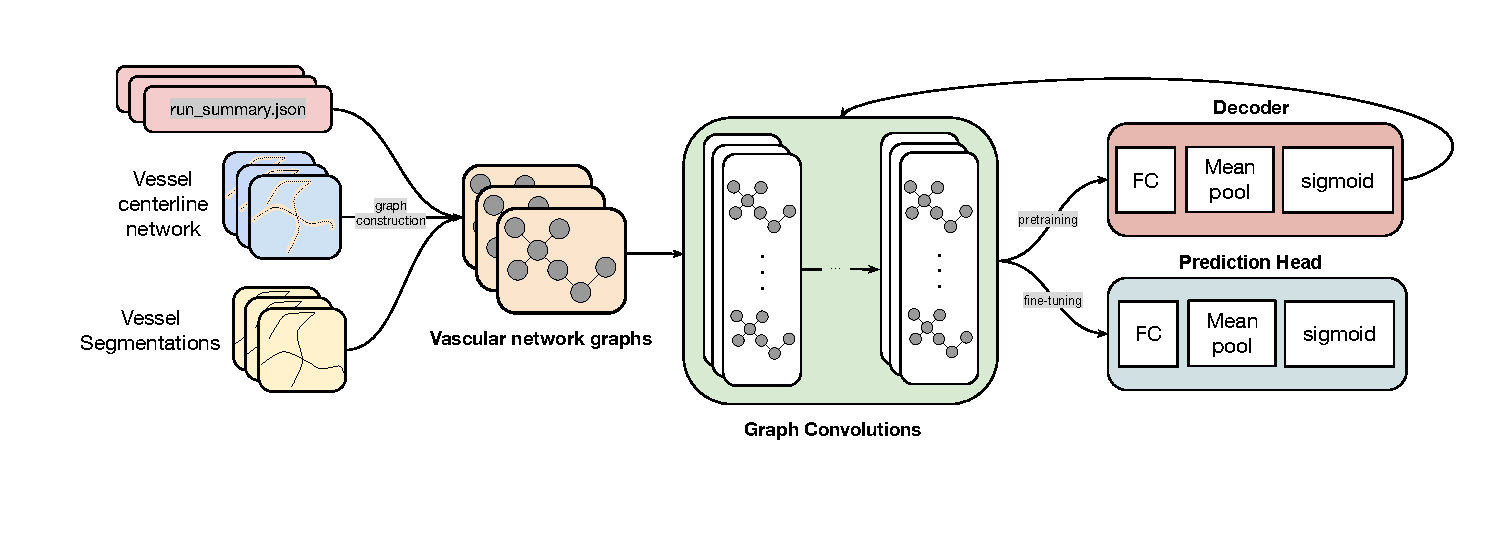
\includegraphics[width=\linewidth]{figures/GNN_arch.pdf}
      \caption{GNN architecture: 4D DCE-MRI through the vessel graph to a pCR
      probability.}
    \end{figure}

  \end{block}

  \begin{block}{Self-supervised Pretraining}

    To improve the performance of the GNN, we use a \textbf{self-supervised pretraining}
    approach. The GNN is first trained to predict \emph{per node} the future contrast
    enhancement, where it learns to predict contrast flow through the network.

    Each contrast curve is cut into non-overlapping windows. Shown the frames on an
    input horizon $[t_1, t_L]$, the model predicts every node's enhancement over the
    following horizon $(t_L, t_{L+H}]$, scored by mean absolute error against the
    measured signal. Predictions are conditioned on \textbf{elapsed seconds}
    $\tau = t - t_1$ rather than on frame index, so the irregular ultrafast cadence
    is handled directly.

  \end{block}

\end{column}

\separatorcolumn

\begin{column}{\colwidth}

  \begin{exampleblock}{Results}

    A different kind of highlighted block.

    $$
    \int_{-\infty}^{\infty} e^{-x^2}\,dx = \sqrt{\pi}
    $$

    Interdum et malesuada fames $\{1, 4, 9, \ldots\}$ ac ante ipsum primis in
    faucibus. Cras eleifend dolor eu nulla suscipit suscipit. Sed lobortis non
    felis id vulputate.

    \heading{A heading inside a block}

    Praesent consectetur mi $x^2 + y^2$ metus, nec vestibulum justo viverra
    nec. Proin eget nulla pretium, egestas magna aliquam, mollis neque. Vivamus
    dictum $\mathbf{u}^\intercal\mathbf{v}$ sagittis odio, vel porta erat
    congue sed. Maecenas ut dolor quis arcu auctor porttitor.

    \heading{Another heading inside a block}

    Sed augue erat, scelerisque a purus ultricies, placerat porttitor neque.
    Donec $P(y \mid x)$ fermentum consectetur $\nabla_x P(y \mid x)$ sapien
    sagittis egestas. Duis eget leo euismod nunc viverra imperdiet nec id
    justo.

  \end{exampleblock}

  \begin{block}{Reproducibility}
    In an effort to promote reproducibility and transparency in our research,
    we have made our code publicly available on GitHub. The 
    repository includes the code for the vessel segmentation, graph construction,'
    GNN training, and evaluation, as well as instructions for how to 
    reproduce our results. 
  \end{block}

  \begin{block}{Conclusion}

    In this study, we proposed a novel approach for predicting treatment response
    in patients with LABC using ultrafast breast MRI scans and GNNs. Our method 
    demonstrates the ability to predict pCR from the vascular 
    network of the tumor, and that self-supervised pretraining can improve the 
    performance of the GNN. Our results suggest that GNNs can be a powerful tool 
    for predicting treatment response in breast cancer, and may have important 
    implications for personalized treatment planning.

   
  \end{block}

  \begin{block}{References}

    \nocite{*}
    \footnotesize{\bibliographystyle{plainnat}\bibliography{poster}}

  \end{block}

\end{column}

\separatorcolumn
\end{columns}
\end{frame}

\end{document}
